\documentclass[a4paper, 12pt]{article}
\usepackage{amsmath}
\usepackage{pgfplots}
\usepackage{tabularx}
\usepgfplotslibrary{dateplot}

\newcommand{\templates}{../../template}
\usepackage[a4paper, margin=2.5cm]{geometry}

\usepackage{enumitem}
\setlist[itemize]{noitemsep}
\setlist[enumerate]{noitemsep}

\let\oldpar\paragraph
\renewcommand{\paragraph}[1]{\oldpar{#1\\}\noindent}
\usepackage{graphicx}
\usepackage{hyperref}
\usepackage{makecell}

\newcommand{\settitolo}[1]{\newcommand{\titolo}{#1\\}}
\newcommand{\setprogetto}[1]{\newcommand{\progetto}{#1\\}}
\newcommand{\setcommittenti}[1]{\newcommand{\committenti}{#1\\}}
\newcommand{\setredattori}[1]{\newcommand{\redattori}{#1\\}}
\newcommand{\setrevisori}[1]{\newcommand{\revisori}{#1\\}}
\newcommand{\setresponsabili}[1]{\newcommand{\responsabili}{#1\\}}
\newcommand{\setversione}[1]{
	\ifdefined\versione\renewcommand{\versione}{#1\\}
	\else\newcommand{\versione}{#1\\}\fi
}
\newcommand{\setdestuso}[1]{\newcommand{\uso}{#1\\}}
\newcommand{\setdescrizione}[1]{\newcommand{\descrizione}{#1\\}}

\newcommand{\makefrontpage}{
	\begin{titlepage}
		\begin{center}

		
\includegraphics[width=0.4\textwidth]{../../template/WSWS-logos_transparent_crop}\\

		{\Large Winning Software Solution}\\[6pt]
		\href{mailto://winningsoftwaresolution@gmail.com}{winningsoftwaresolution@gmail.com}\\
		
		\ifdefined\progetto
		\vspace{1cm}
		{\Large\progetto}
		{\large\committenti}
		\else\fi
		
		\vspace{1.5cm}
		{\LARGE\titolo}
		
		\vfill
		
		\begin{tabular}{r | l}
		\multicolumn{2}{c}{\textit{Informazioni}}\\
		\hline
		
		\ifdefined\redattori
			\textit{Redattori} &
			\makecell[l]{\redattori}\\
		\else\fi
		\ifdefined\revisori
			\textit{Revisori} &
			\makecell[l]{\revisori}\\
		\else\fi
		\ifdefined\responsabili
			\textit{Respondabili} &
			\makecell[l]{\responsabili}\\
		\else\fi
		
		\ifdefined\versione
			\textit{Versione} & \versione
		\else\fi
		
		\textit{Uso} & \uso
		
		\end{tabular}
		
		\vspace{2cm}
		
		\ifdefined\descrizione
		Descrizione
		\vspace{6pt}
		\hrule
		\descrizione
		\else\fi
		\end{center}
	\end{titlepage}
}
\usepackage{hyperref}
\usepackage{array}
\usepackage{tabularx}

\def\vers#1-#2-#3-#4-#5\\{#1&#2&#3&#4&#5\\\hline}

\newcommand{\addversione}[5]{
	\ifdefined\versioni
		\let\old\versioni
		\renewcommand{\versioni}{#1&#2&#3&#4&#5\\\hline\old}
	\else
		\newcommand{\versioni}{#1&#2&#3&#4&#5\\\hline}
	\fi
}

\newcommand{\setversioni}[1]{\newcommand{\versioni}{#1}}

\newcommand{\makeversioni}{
	\begin{center}
		\begin{tabularx}{\textwidth}{|c|c|c|c|X|}
		\hline
		\textbf{Versione} & \textbf{Data} & \textbf{Persona} & \textbf{Attivtà} & \textbf{Descrizione} \\
		\hline
		\versioni
		\end{tabularx}
	\end{center}
	\clearpage
}

\settitolo{Piano di Qualifica}
\setredattori{Raffaele Oliviero \\ Elia Scandaletti \\ Giovanni Cocco}
\setdestuso{esterno}
\setdescrizione{
Questo documento serve a definire le metriche e i criteri di accettazione dei prodotti.
}

\addversione{0.0.0}{09/01/2021}{Raffaele Oliviero}{Redazione}{Stesura iniziale.}
\addversione{0.0.1}{16/01/2021}{Elia Scandaletti}{Redazione}{Correzione indice di Gulpease.}
\addversione{0.0.2}{16/01/2021}{Giovanni Cocco}{Redazione}{Migliorata la leggibilità.}
\addversione{0.0.3}{04/02/2021}{Giovanni Cocco}{Redazione}{Stesura iniziale sezione software.}
\addversione{0.0.4}{21/02/2021}{Giovanni Cocco}{Redazione}{Aggiunta dashboard al docuemento.}
\addversione{2.0.0}{23/03/2021}{Elia Scandaletti}{Redazione}{Rifacimento del documento.}


\begin{document}

\makefrontpage

\makeversioni

\tableofcontents
\clearpage

\section{Qualità di prodotto}

\subsection{Documentazione}
\subsubsection{Indice di Gulpease}
\[ \text{Indice di Gulpease} = 89 + \frac{300*\text{\#frasi} - 10*\text{\#lettere}}{\text{\#parole}} \]
\begin{itemize}
	\item \#lettere: numero di caratteri alfanumerici;
	\item \#parole: numero di gruppi di caratteri alfanumerici;
	\item \#frasi: numero di gruppi di punti o punti e virgola consecutivi.
\end{itemize}

\subparagraph{Prodotti coinvolti:}
\begin{center}
	\begin{tabularx}{\textwidth}{|X|X|X|}
		\hline
		\textbf{Prodotto} & \textbf{Valore accettabile} & \textbf{Valore ottimale } \\
		\hline
		Documenti interni & $>$ 40                      & $>$ 60                    \\
		\hline
		Documenti esterni & $>$ 50                      & $>$ 60                    \\
		\hline
	\end{tabularx}\\[8pt]
	\mbox{}\\
\end{center}

\subparagraph{Strumenti utilizzati:}
\begin{itemize}
	\item Python - \texttt{textract}.
\end{itemize}

\subparagraph{Andamento:}
\begin{center}
	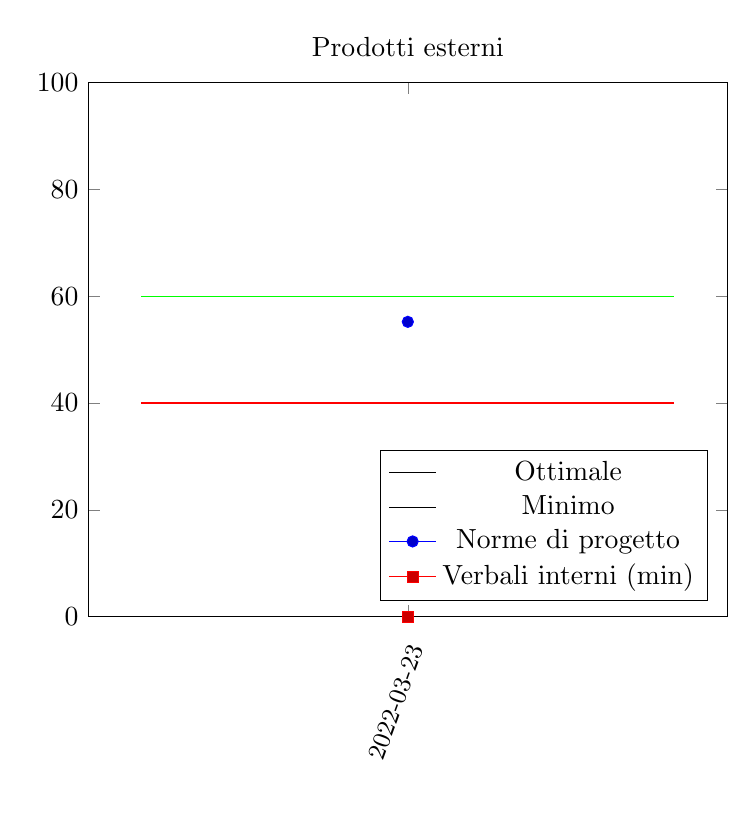
\begin{tikzpicture}
		\pgfplotsset{width=0.8\textwidth}
		\begin{axis}[
				title = {Prodotti esterni},
				axis x line = none,
				axis y line = none,
				ymin = 0, ymax = 100
			]
			\addplot [green]{60}; \label{opt}
			\addplot [red]{40}; \label{min}
		\end{axis}
		\begin{axis}[
				date coordinates in = x,
				xticklabel =	\year-\month-\day,
				x tick label style = {
						font = \small,
						text width = 1.9cm,
						align = center,
						rotate = 70,
						anchor = north east
					},
				xtick = data,
				ymin = 0, ymax = 100,
				legend pos = south east
			]
			\addlegendimage{/pgfplots/refstyle=opt}
			\addlegendentry{Ottimale}
			\addlegendimage{/pgfplots/refstyle=min}
			\addlegendentry{Minimo}
			\addplot coordinates {
					(2022-03-23, 55.2)
				};\addlegendentry{Norme di progetto}

			\addplot coordinates {
					(2022-03-23, 0)
				};\addlegendentry{Verbali interni (min)}
		\end{axis}
	\end{tikzpicture}
\end{center}

\begin{center}
	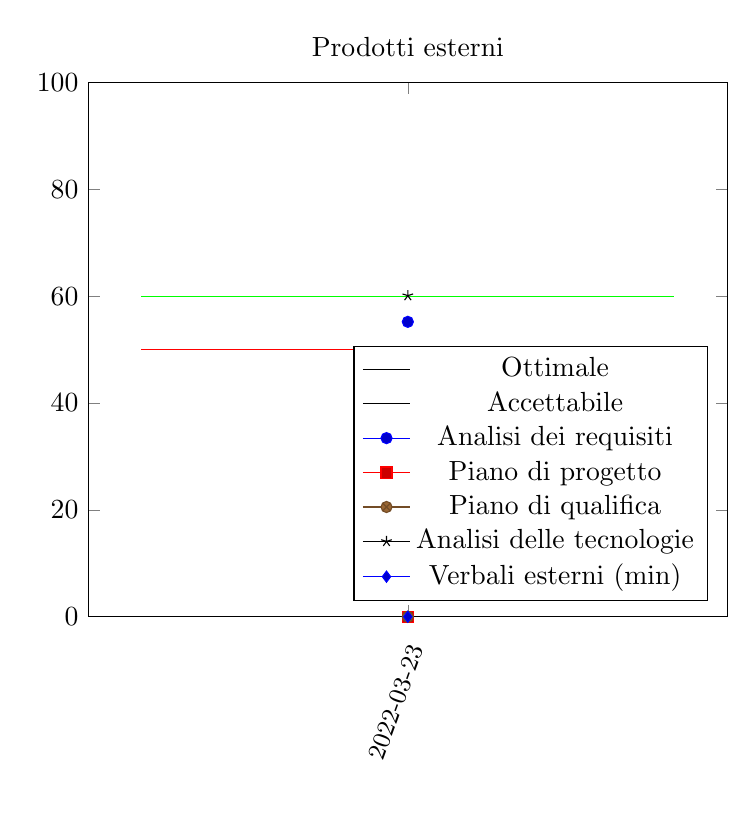
\begin{tikzpicture}
		\pgfplotsset{width=0.8\textwidth}
		\begin{axis}[
				title = {Prodotti esterni},
				axis x line = none,
				axis y line = none,
				ymin = 0, ymax = 100
			]
			\addplot [green]{60}; \label{opt}
			\addplot [red]{50}; \label{min}
		\end{axis}
		\begin{axis}[
				date coordinates in = x,
				xticklabel =	\year-\month-\day,
				x tick label style = {
						font = \small,
						text width = 1.9cm,
						align = center,
						rotate = 70,
						anchor = north east
					},
				xtick = data,
				ymin = 0, ymax = 100,
				legend pos = south east
			]
			\addlegendimage{/pgfplots/refstyle=opt}
			\addlegendentry{Ottimale}
			\addlegendimage{/pgfplots/refstyle=min}
			\addlegendentry{Accettabile}
			\addplot coordinates {
					(2022-03-23, 55.2)
				};\addlegendentry{Analisi dei requisiti}

			\addplot coordinates {
					(2022-03-23, 0)
				};\addlegendentry{Piano di progetto}

			\addplot coordinates {
					(2022-03-23, 0)
				};\addlegendentry{Piano di qualifica}

			\addplot coordinates {
					(2022-03-23, 60.1)
				};\addlegendentry{Analisi delle tecnologie}

			\addplot coordinates {
					(2022-03-23, 0)
				};\addlegendentry{Verbali esterni (min)}
		\end{axis}
	\end{tikzpicture}
\end{center}

\subparagraph{Riferimenti:} \underline{\href{http://www.corrige.it/leggibilita/lindice-gulpease/}{http://www.corrige.it/leggibilita/lindice-gulpease/}}

\subsection{Prodotti software}

\subsubsection{Copertura statement}
La metrica si basa sullo statement coverage.

\subparagraph{Prodotti coinvolti:}
\begin{center}
	\begin{tabularx}{\textwidth}{|X|X|X|}
		\hline
		\textbf{Prodotto} & \textbf{Valore accettabile } & \textbf{Valore ottimale } \\
		\hline
		Software          & $>$ 80\%                     & 100\%                     \\
		\hline
	\end{tabularx}\\[8pt]
	\mbox{}\\
\end{center}

\subparagraph{Strumenti utilizzati:} \begin{itemize}
	\item Jest;
	\item JSCoverage;
	\item PyTest;
	\item truffle.
\end{itemize}

\subparagraph{Andamento:}
\begin{center}
	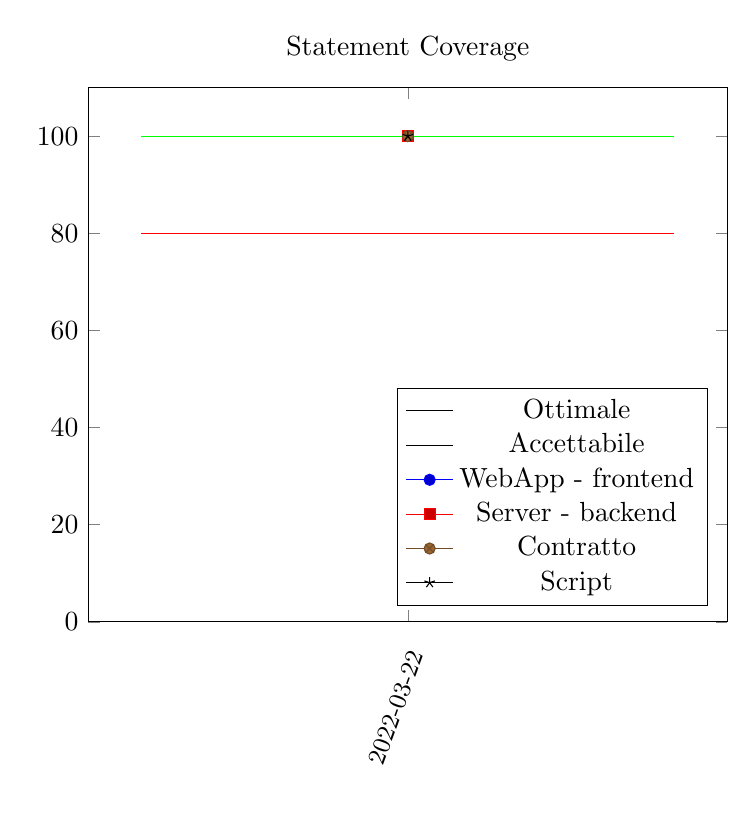
\begin{tikzpicture}
		\pgfplotsset{width=0.8\textwidth}
		\begin{axis}[
				title = {Statement Coverage},
				axis x line = none,
				axis y line = none,
				ymin = 0, ymax = 110
			]
			\addplot [green]{100}; \label{opt}
			\addplot [red]{80}; \label{min}
		\end{axis}
		\begin{axis}[
				date coordinates in = x,
				xticklabel =	\year-\month-\day,
				x tick label style = {
						font = \small,
						text width = 1.9cm,
						align = center,
						rotate = 70,
						anchor = north east
					},
				xtick = data,
				ymin = 0, ymax = 110,
				legend pos = south east
			]
			\addlegendimage{/pgfplots/refstyle=opt}
			\addlegendentry{Ottimale}
			\addlegendimage{/pgfplots/refstyle=min}
			\addlegendentry{Accettabile}
			\addplot coordinates {
					(2022-03-22, 10)
				};\addlegendentry{WebApp - frontend}
			\addplot coordinates {
					(2022-03-22, 100)
				};\addlegendentry{Server - backend}
			\addplot coordinates {
					(2022-03-22, 100)
				};\addlegendentry{Contratto}
			\addplot coordinates {
					(2022-03-22, 100)
				};\addlegendentry{Script}
		\end{axis}
	\end{tikzpicture}
\end{center}

\subsubsection{Copertura branch}
La metrica si basa sullo branch coverage.

\subparagraph{Prodotti coinvolti:}
\begin{center}
	\begin{tabularx}{\textwidth}{|X|X|X|}
		\hline
		\textbf{Prodotto} & \textbf{Valore accettabile } & \textbf{Valore ottimale } \\
		\hline
		Software          & $>$ 80\%                     & 100\%                     \\
		\hline
	\end{tabularx}\\[8pt]
	\mbox{}\\
\end{center}

\subparagraph{Strumenti utilizzati:} \begin{itemize}
	\item Jest;
	\item JSCoverage;
	\item PyTest;
	\item truffle.
\end{itemize}

\subparagraph{Andamento:}
\begin{center}
	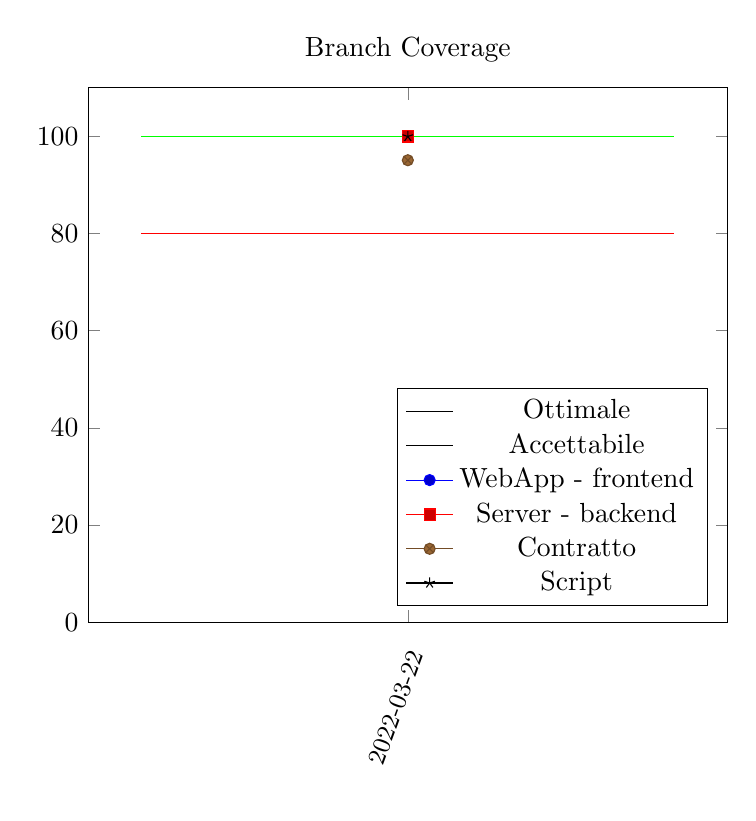
\begin{tikzpicture}
		\pgfplotsset{width=0.8\textwidth}
		\begin{axis}[
				title = {Branch Coverage},
				axis x line = none,
				axis y line = none,
				ymin = 0, ymax = 110
			]
			\addplot [green]{100}; \label{opt}
			\addplot [red]{80}; \label{min}
		\end{axis}
		\begin{axis}[
				date coordinates in = x,
				xticklabel =	\year-\month-\day,
				x tick label style = {
						font = \small,
						text width = 1.9cm,
						align = center,
						rotate = 70,
						anchor = north east
					},
				xtick = data,
				ymin = 0, ymax = 110,
				legend pos = south east
			]
			\addlegendimage{/pgfplots/refstyle=opt}
			\addlegendentry{Ottimale}
			\addlegendimage{/pgfplots/refstyle=min}
			\addlegendentry{Accettabile}
			\addplot coordinates {
					(2022-03-22, 10)
				};\addlegendentry{WebApp - frontend}
			\addplot coordinates {
					(2022-03-22, 100)
				};\addlegendentry{Server - backend}
			\addplot coordinates {
					(2022-03-22, 95.1)
				};\addlegendentry{Contratto}
			\addplot coordinates {
					(2022-03-22, 100)
				};\addlegendentry{Script}
		\end{axis}
	\end{tikzpicture}
\end{center}

\section{Qualità di processo}
\subsubsection{Time variance}
La metrica si basa sulla variazione percentuale rispetto alla stima iniziale.

\subparagraph{Prodotti coinvolti:}
\begin{center}
	\begin{tabularx}{\textwidth}{|X|X|X|}
		\hline
		\textbf{Prodotto} & \textbf{Valore accettabile } & \textbf{Valore ottimale } \\
		\hline
		Software          & $<$ 20\%                     & 0\%                       \\
		\hline
		Documentazione    & $<$ 20\%                     & 0\%                       \\
		\hline
	\end{tabularx}\\[8pt]
	\mbox{}\\
\end{center}

\subparagraph{Andamento:}
\begin{center}
	\begin{tikzpicture}
		\pgfplotsset{width=0.8\textwidth}
		\begin{axis}[
				title = {Time variance},
				axis x line = none,
				axis y line = none,
				ymin = -10, ymax = 110
			]
			\addplot [green]{0}; \label{opt}
			\addplot [red]{20}; \label{min}
		\end{axis}
		\begin{axis}[
				date coordinates in = x,
				xticklabel =	\year-\month-\day,
				x tick label style = {
						font = \small,
						text width = 1.9cm,
						align = center,
						rotate = 70,
						anchor = north east
					},
				xtick = data,
				ymin = -10, ymax = 110
			]
			\addlegendimage{/pgfplots/refstyle=opt}
			\addlegendentry{Ottimale}
			\addlegendimage{/pgfplots/refstyle=min}
			\addlegendentry{Accettabile}
			\addplot coordinates {
					(2022-03-22, 0)
				};\addlegendentry{Documenti}
			\addplot coordinates {
					(2022-03-22, 0)
				};\addlegendentry{Software}
		\end{axis}
	\end{tikzpicture}
\end{center}

\subsubsection{Budget variance}
La metrica si basa sulla variazione percentuale rispetto alla stima iniziale.

\subparagraph{Prodotti coinvolti:}
\begin{center}
	\begin{tabularx}{\textwidth}{|X|X|X|}
		\hline
		\textbf{Prodotto} & \textbf{Valore accettabile } & \textbf{Valore ottimale } \\
		\hline
		Software          & $<$ 20\%                     & 0\%                       \\
		\hline
		Documentazione    & $<$ 20\%                     & 0\%                       \\
		\hline
	\end{tabularx}\\[8pt]
	\mbox{}\\
\end{center}

\subparagraph{Andamento:}
\begin{center}
	\begin{tikzpicture}
		\pgfplotsset{width=0.8\textwidth}
		\begin{axis}[
				title = {Budget variance},
				axis x line = none,
				axis y line = none,
				ymin = -10, ymax = 110
			]
			\addplot [green]{0}; \label{opt}
			\addplot [red]{20}; \label{min}
		\end{axis}
		\begin{axis}[
				date coordinates in = x,
				xticklabel =	\year-\month-\day,
				x tick label style = {
						font = \small,
						text width = 1.9cm,
						align = center,
						rotate = 70,
						anchor = north east
					},
				xtick = data,
				ymin = -10, ymax = 110
			]
			\addlegendimage{/pgfplots/refstyle=opt}
			\addlegendentry{Ottimale}
			\addlegendimage{/pgfplots/refstyle=min}
			\addlegendentry{Accettabile}
			\addplot coordinates {
					(2022-03-22, 0)
				};\addlegendentry{Documenti}
			\addplot coordinates {
					(2022-03-22, 0)
				};\addlegendentry{Software}
		\end{axis}
	\end{tikzpicture}
\end{center}
\end{document}